
%======================================================================
\documentclass{beamer}
%----------------------------------------------------------------------
\newcommand{\Code}[1]{\textsf{#1}}
\newcommand{\cello}{\textsf{Cello}}
\newcommand{\enzo}{\textsf{Enzo}}
%----------------------------------------------------------------------
\usetheme{Copenhagen}
\usecolortheme{default}
%----------------------------------------------------------------------
% \usepackage{color}
% \usepackage{graphics}
% \usepackage{wasysym}
%----------------------------------------------------------------------
\newcommand{\code}[1]{\texttt{#1}}
\newcommand{\good}{\textcolor{green}{\smiley}}
\newcommand{\bad}{\textcolor{red}{\frownie}}
\newcommand{\colorcode}[1]{\textcolor{blue}{\code{#1}}}
%======================================================================

\title[The \cello\ Project]
      {The \cello\ Project \\ \small{Enzo: The Next Generation}}

\author[James Bordner]{\small Laboratory for Computational Astrophysics \\ San Diego Supercomputer Center \\ University of California, San Diego \\ \ \\ James Bordner}

\date{\today}

\begin{document}



%----------------------------------------------------------------------
\begin{frame}
\titlepage
\end{frame}
%----------------------------------------------------------------------


% \input{slide-perf-motivation}

%========================================================================
\part{Overview}
%========================================================================

\section{Overview}

%----------------------------------------------------------------------
\begin{frame}
\frametitle{Outline}

\begin{enumerate}
\item Overview
\item Related Work
\item User's Perspective
\item Designer's Perspective
\item Data Structures
\end{enumerate}
\end{frame}
%----------------------------------------------------------------------

%----------------------------------------------------------------------
\begin{frame}
\frametitle{Goals}

\begin{itemize}
\item \enzo: The Next Generation
\item Computational Science tool for next 10+ years
\item Many competing design goals:
\begin{itemize}
\item Easy to use, modify, maintain
\item Scalable to O($10^{5+}$)  cores
\item Adaptable to evolving hardware and middleware
\item Quality control
\item \textit{Science capabilities}
\end{itemize}
\end{itemize}
\end{frame}
%----------------------------------------------------------------------

%----------------------------------------------------------------------
\begin{frame}
\frametitle{Target Classes of Users}
\begin{itemize}
\item \textbf{Students}
\begin{itemize}
\item easy to define problem, run, and analyse
\item minimal software-related ``gotcha's''
\end{itemize}
\item \textbf{Physics experts}
\begin{itemize}
\item deep control of physics parameters
\item flexible problem set up for wide range of problems
\end{itemize}
\item \textbf{Numerical experts}
\begin{itemize}
\item deep control of method parameters
\item easy to incorporate new methods
\end{itemize}
\item \textbf{Computing experts}
\begin{itemize}
\item deep control of data structures
\item AMR, parallelization, data distribution, blocking/padding
\end{itemize}
\end{itemize}
\end{frame}
%----------------------------------------------------------------------

%----------------------------------------------------------------------
\begin{frame}
\frametitle{Target Classes of Problems}

\begin{itemize}
\item More AMR $\rightarrow$ more data dependencies $\rightarrow$ less parallelism
\item \textbf{Single-resolution (``unigrid'')}
\begin{itemize}
\item Parallelizes fully
\item \enzo\ does well, but still room for improvement
\end{itemize}
\item \textbf{Shallow multi-resolution}
\item \textbf{Deep multi-resolution}
\item \textbf{\textit{Extreme} multi-resolution}
\begin{itemize}
\item Most difficult to parallelize effectively
\item \enzo\ does not scale well with hierarchy depth
\end{itemize}
\end{itemize}
\end{frame}
%----------------------------------------------------------------------

%----------------------------------------------------------------------
\begin{frame}
\frametitle{Summary of changes compared to \enzo}
\begin{itemize}
\item Overhauled parallel distributed data structures
\item Improved AMR approach(es)
\begin{itemize}
\item  Patch-based and tree-based AMR have advantages/disadvantages
\item  Implement both
\end{itemize}
\item Improved definition and control of parallel tasks
\begin{itemize}
\item Maintain pool of parallel tasks (CHARM++?)
\item Flexible data distribution
\item Smarter  data re-distribution
\item Multiple choices for parallelism (MPI-[12], OMP, UPC)
\end{itemize}
\item Improved problem specification scope and depth of control
\item More rigorous software development methodology
\end{itemize}

\end{frame}
%----------------------------------------------------------------------

%========================================================================
\part{Related Work}
%========================================================================

\section{SAGE/RAGE}

\section{Paramesh / Flash}

%----------------------------------------------------------------------
\begin{frame}
\frametitle{Paramesh}
\centerline{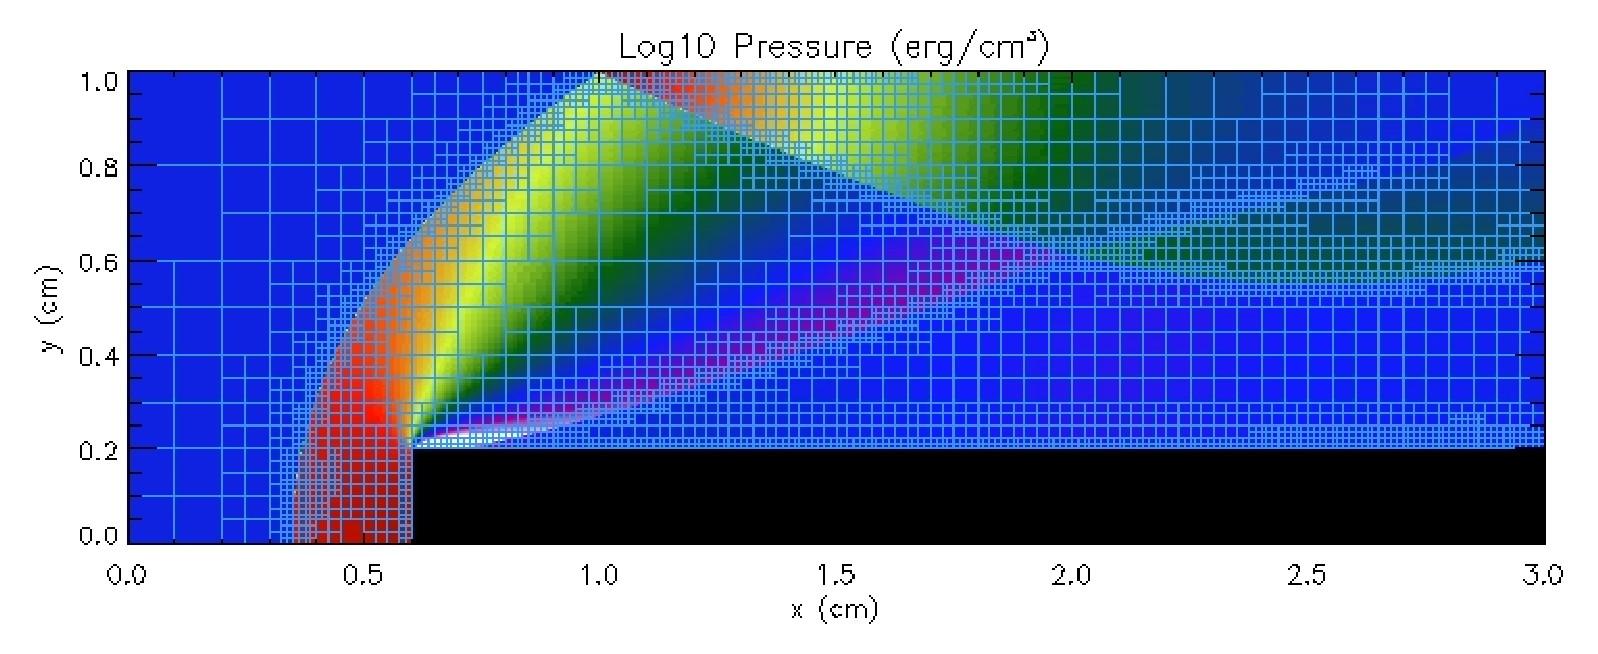
\includegraphics[width=4in]{paramesh.eps}}
\end{frame}
%----------------------------------------------------------------------


\section{Chombo}

%========================================================================
\part{User's Perspective}
%========================================================================

\section{Parameter Files}


%========================================================================
\part{Designer's Perspective}
%========================================================================

%========================================================================
\part{Data Structures}
%========================================================================

\section{Cello Components}

%----------------------------------------------------------------------
\begin{frame}
\frametitle{Components}
\centerline{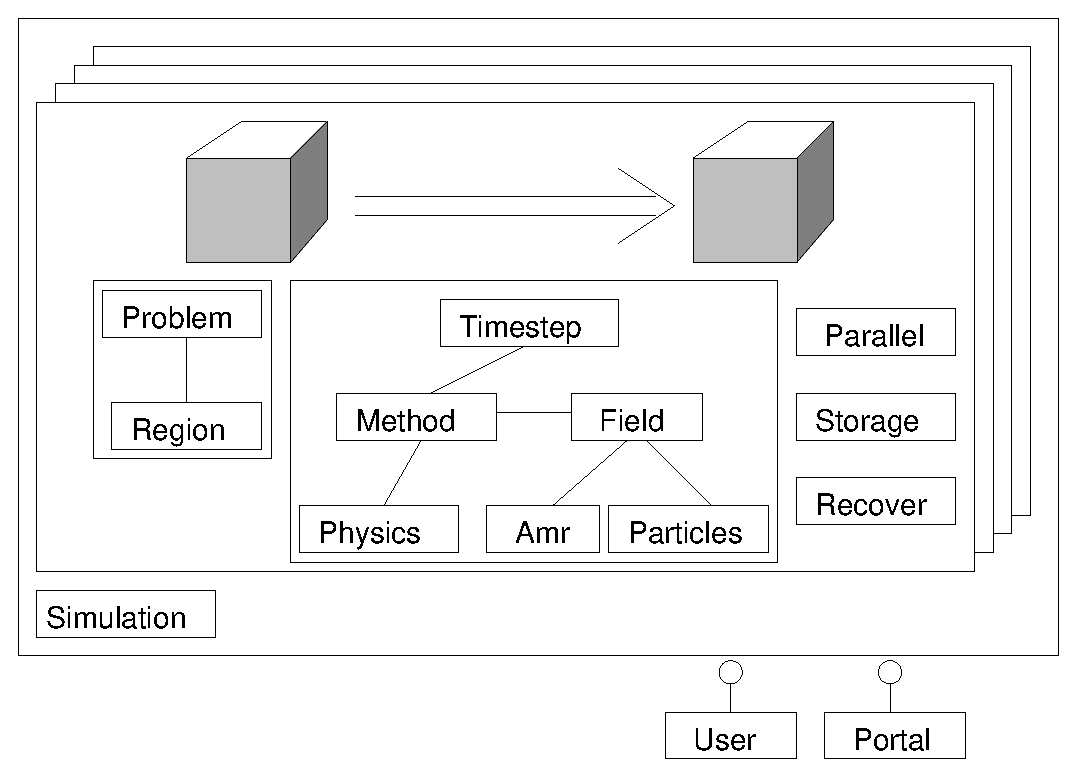
\includegraphics[width=3in]{components.eps}}
\end{frame}
%----------------------------------------------------------------------

\section{\code{Array} class}

%----------------------------------------------------------------------
\begin{frame}
\frametitle{\code{Array} class}

\begin{itemize}
\item Conceptually a Fortran-like array
\item Data distributed via MPI-[12], OMP, [UPC]
\item Data layout may be blocked / padded for cache
\item Interface between high-level C++ and low-level Fortran/C
\end{itemize}
\end{frame}
%----------------------------------------------------------------------

%----------------------------------------------------------------------
\begin{frame}
\frametitle{\code{Array} class}

\begin{minipage}{1.8in}
\begin{itemize}
\item[]<1->
\includegraphics[width=0.4in]{array-serial.eps} \ \ \code{ArraySerial}
\item[]<2-> 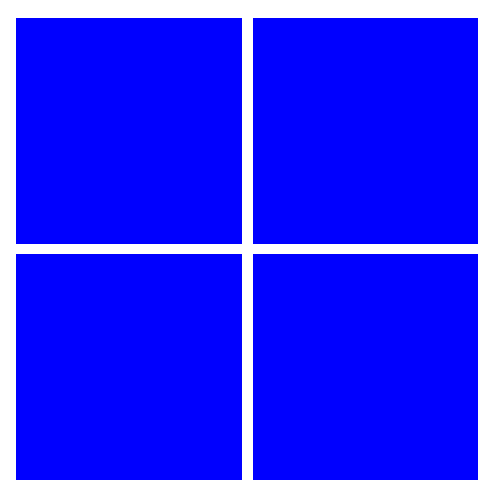
\includegraphics[width=0.4in]{array-block.eps} \ \ \code{ArrayBlock}
\item[]<3-> 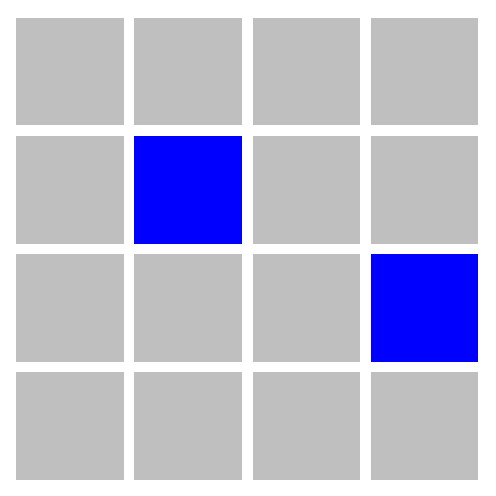
\includegraphics[width=0.4in]{array-mpi.eps} \ \ \code{ArrayMpi}
\end{itemize}
\end{minipage} \ 
\begin{minipage}{2in}
\begin{itemize}
\item[]<4-> 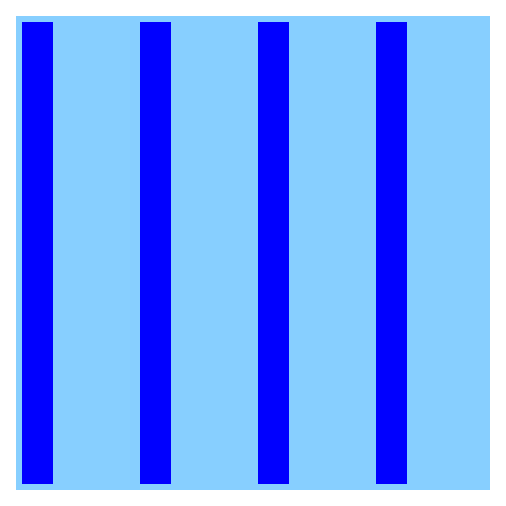
\includegraphics[width=0.4in]{array-omp.eps} \ \ \code{ArrayOmp}
\item[]<5-> 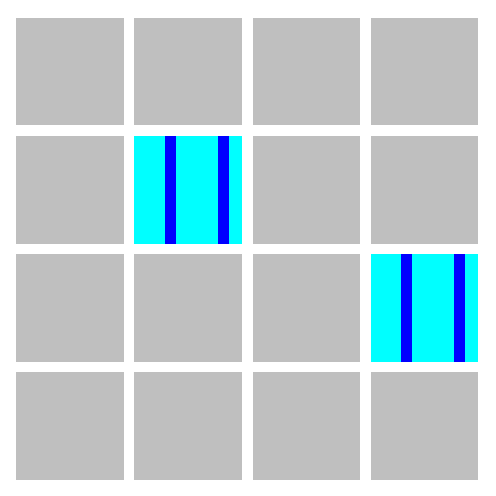
\includegraphics[width=0.4in]{array-mpi-omp.eps} \ \ \code{ArrayMpiOmp}
\item[]<6-> 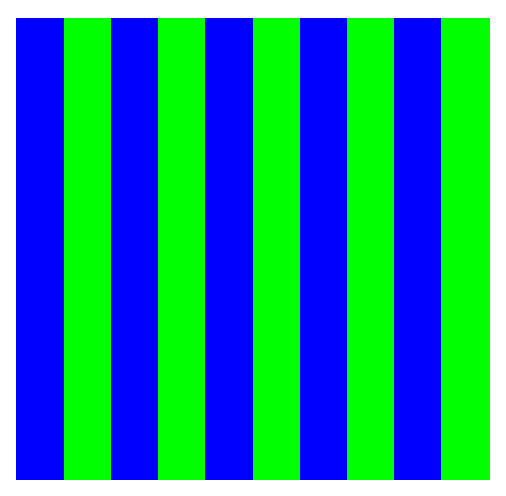
\includegraphics[width=0.4in]{array-interleave.eps} \ \ \code{ArrayInterleave}
\end{itemize}
\end{minipage}

\end{frame}
%----------------------------------------------------------------------

\section{\code{Amr} class}

%----------------------------------------------------------------------
\begin{frame}
\frametitle{Patch-AMR Versus Tree-AMR}

\end{frame}
%----------------------------------------------------------------------




%----------------------------------------------------------------------
\begin{frame}
\frametitle{}

\end{frame}
%----------------------------------------------------------------------

\end{document}

